\section{}
Z wykorzystaniem płytki UC-1, oraz układów 7400 i 7410 zbudowano synchroniczny przerzutnik RS.
Zbadano działanie przerzutnika podając na wejście zegarowe sygnał z impulsatora, ustawiając uprzednio stany wejść informacyjnych, oraz śledząc jednocześnie stan wyjścia układu za pomocą próbnika stanów logicznych obecnego na płytce UC-1.

Zaobserwowane działanie przerzutnika było zgodne z oczekiwanym.
Wejścia c oraz d pełnią rolę sygnałów \textit{preset} oraz \textit{clear}, pozwalając na asynchroniczną zmianę stanu przerzutnika.

\begin{table}[H]
    \centering
    \begin{tabular}{c|c|c|c|c||c|c}
        \hline
        zegar & a     & b     & c & d & \(Q_{n+1}\) & \(\overline{Q_{n+1}}\)
        \\ \hline\hline
        1     & 0     & 0     & 1 & 1 & \(Q_n\)     & \(\overline{Q_n}\)     \\ \hline
        1     & 0     & 1     & 1 & 1 & 0           & 1                      \\ \hline
        1     & 1     & 0     & 1 & 1 & 1           & 0                      \\ \hline
        0     & \(-\) & \(-\) & 1 & 1 & \(Q_n\)     & \(\overline{Q_n}\)     \\ \hline
        \(-\) & \(-\) & \(-\) & 0 & 1 & 1           & 0                      \\ \hline
        \(-\) & \(-\) & \(-\) & 1 & 0 & 0           & 1                      \\ \hline
    \end{tabular}
    \caption{Tabela prawdy dozwolonych stanów badanego synchronicznego przerzutnika RS.}
\end{table}

\begin{figure}[H]
    \centering
    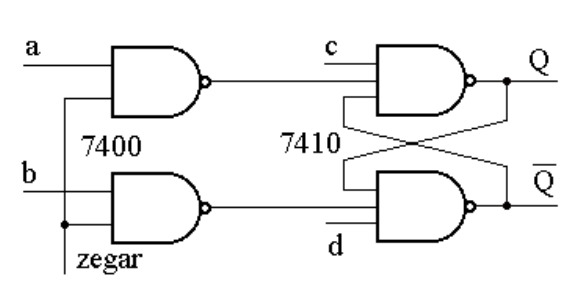
\includegraphics[width=7.5cm]{include/1/1.png}
    \caption{Schemat zbudowanego synchronicznego przerzutnika RS.}
\end{figure}